% !TEX enableShellEscape = yes
% (The above line makes atom's latex package compile with -shell-escape
% for minted, and is just ignored by other systems.)
\documentclass{article}

\usepackage{fullpage}
\usepackage{color}
\usepackage{amsmath,amssymb}
\usepackage{url}
\usepackage{verbatim}
\usepackage{graphicx}
\usepackage{parskip}
\usepackage{amssymb}
\usepackage{hyperref}

% Use one or the other of these for displaying code.
% NOTE: If you get
%  ! Package minted Error: You must invoke LaTeX with the -shell-escape flag.
% and don't want to use minted, just comment out the next line
\usepackage{minted} \BeforeBeginEnvironment{minted}{\begingroup\color{black}} \AfterEndEnvironment{minted}{\endgroup} \setminted{autogobble,breaklines,breakanywhere,linenos}

\usepackage{listings}

% Colours
\definecolor{blu}{rgb}{0,0,1}
\newcommand{\blu}[1]{{\textcolor{blu}{#1}}}
\definecolor{gre}{rgb}{0,.5,0}
\newcommand{\gre}[1]{\textcolor{gre}{#1}}
\definecolor{red}{rgb}{1,0,0}
\newcommand{\red}[1]{\textcolor{red}{#1}}
\definecolor{pointscolour}{rgb}{0.6,0.3,0}

% answer commands
\newcommand\ans[1]{\par\gre{Answer: #1}}
\newenvironment{answer}{\par\begingroup\color{gre}Answer: }{\endgroup}
\let\ask\blu
\let\update\red
\newenvironment{asking}{\begingroup\color{blu}}{\endgroup}
\newcommand\pts[1]{\textcolor{pointscolour}{[#1~points]}}

% Math
\def\R{\mathbb{R}}
\DeclareMathOperator*{\argmax}{arg\,max}
\DeclareMathOperator*{\argmin}{arg\,min}
\newcommand{\norm}[1]{\lVert #1 \rVert}
\newcommand{\mat}[1]{\begin{bmatrix}#1\end{bmatrix}}

% LaTeX
\newcommand{\fig}[2]{\includegraphics[width=#1\textwidth]{#2}}
\newcommand{\centerfig}[2]{\begin{center}\includegraphics[width=#1\textwidth]{#2}\end{center}}

\begin{document}

\title{CPSC 340 Assignment 3 (see course page for due date)}
\date{}
\maketitle


\vspace{-4em}



\section*{Important: Submission Format \pts{5}}

    Please make sure to follow the submission instructions posted on the course website.
    \ask{We will deduct marks if the submission format is incorrect, or if you're not using \LaTeX{} and your handwriting is \emph{at all} difficult to read} -- at least these 5 points, more for egregious issues.
    Compared to assignment 1, your name and student number are no longer necessary (though it's not a bad idea to include them just in case, especially if you're doing the assignment with a partner).


\section{Matrix Notation and Minimizing Quadratics \pts{12}}


\subsection{Converting to Matrix/Vector/Norm Notation \pts{6}}

Using our standard supervised learning notation ($X$, $y$, $w$)
\ask{express the following functions in terms of vectors, matrices, and norms} (there should be no summations or maximums).
\begin{enumerate}
\item $\max_{i \in \{1,2,\dots,n\}}  |w^Tx_i - y_i|$. This is ``brittle regression''.
\begin{answer}
	\begin{equation}
		\text{Let} \quad r = | X w - y |
	\end{equation}
	Then the funciton can be expressed as $\max_i r_i$
\end{answer}
\item $\sum_{i=1}^n v_i(w^Tx_i  - y_i)^2 + \frac{\lambda}{2}\sum_{j=1}^d w_j^2$. This is regularized least squares with a \emph{weight} $v_i$ for each training example:  Hint: You can use $V$ to denote a diagonal matrix that has the values $v_i$ along the diagonal. What does $a^T V b$ look like in summation form (for some arbitrary vectors $a$, $b$)?
\begin{answer}
	Let $V$ denote a diagonal matrix with values $v_{i}$.
	\begin{equation}
		(X w - y)^{T} V (X w - y) + \frac{\lambda}{2} w^{T} w
	\end{equation}
\end{answer}

\item $\left(\sum_{i=1}^n |w^Tx_i - y_i|\right)^2 +  \frac12 \sum_{j=1}^{d} \lambda_j|w_j|$. This is L1-regularized least squares with a different regularization strength for each dimension: Hint: You can use  $\Lambda$ to denote a diagonal matrix that has the $\lambda_j$ values along the diagonal.
\begin{answer}
	Denote a veter $A = [1,1,....]^{T}$
	\begin{equation}
		((X w - y)^{T} A)^2 + |w| \Lambda A
	\end{equation}
	
\end{answer}
\end{enumerate}

Note: you can assume that all the $v_i$ and $\lambda_i$ values are non-negative.

\subsection{Minimizing Quadratic Functions as Linear Systems \pts{6}} \label{sec:lin-sys}

\ask{Write finding a minimizer $w$ of the functions below as a system of linear equations} (using vector/matrix notation and simplifying as much as possible). Note that all the functions below are convex, so finding a $w$ with $\nabla f(w) = 0$ is sufficient to minimize the functions -- but show your work in getting to this point.

\begin{enumerate}
\item $f(w) = \frac{1}{2} \norm{w-v}^2$ (projection of $v$ onto real space).
\begin{answer}
	$w = v $
\end{answer}
\item $f(w)= \frac{1}{2} \norm{Xw - y}^2 + \frac{1}{2} w^T\Lambda w$ (least squares with weighted regularization).
\begin{answer}
	\begin{equation}
		f(w) = \frac{1}{2} w^{T} X^{T} X w - w^{T} X^{T} y + \frac{1}{2} y^{T} y + \frac{1}{2} w^T\Lambda w
	\end{equation}
	Therefore,
	\begin{equation}
		\nabla f(w) = X^{T} X w - X^{T}y + \Lambda w = 0
	\end{equation}

	\begin{equation}
		\Rightarrow w = (X^{T} X + \Lambda)^{-1} X^{T}y                  
	\end{equation}
\end{answer}

\item $f(w) = \frac{1}{2} \sum_{i=1}^n v_i (w^Tx_i - y_i)^2 + \frac{\lambda}{2}\norm{w-w^{(0)}}^2$ (weighted least squares shrunk towards non-zero $w^{(0)}$). \label{item:weighted-shrunk-ls}
\begin{answer}
	\begin{equation}
		f(w) = \frac{1}{2}(w^{T}X^{T}VXw - 2w^{T}X^{T}Vy + y^{T}Vy)+ \lambda (w^{T} w - 2 w^{T} w^{(0)} + {w^{(0)}}^{T} w^{(0)})
	\end{equation}

	\begin{equation}
		\nabla f(w) = X^{T}VX w - X^{T}Vy + 2\lambda w - 2\lambda w^{(0)} = 0
	\end{equation}

	\begin{equation}
		\Rightarrow w = (X^{T}VX + 2\lambda I)^{-1} (X^{T}Vy + 2\lambda w^{(0)})
	\end{equation}
\end{answer}
\end{enumerate}
Above we assume that $v$ and $w^{(0)}$ are $d \times 1$ vectors, and $\Lambda$ is a $d \times d$ diagonal matrix (with positive entries along the diagonal). You can use $V$ as a diagonal matrix containing the $v_i$ values along the diagonal.

Hint: Once you convert to vector/matrix notation, you can use the results from class to quickly compute these quantities term-wise.
As a spot check, make sure that the dimensions match for all quantities/operations: to do this, you may need to introduce an identity matrix. For example, $X^T X w + \lambda w$ can be re-written as $(X^T X + \lambda I)w$.


\clearpage
\section{Robust Regression and Gradient Descent \pts{41}}

If you run \verb|python main.py -q 2|, it will load a one-dimensional regression
dataset that has a non-trivial number of `outlier' data points.
These points do not fit the general trend of the rest of the data,
and pull the least squares model away from the main downward trend that most data points exhibit:
\centerfig{.7}{./figs/least_squares_outliers.pdf}

Note: we are fitting the regression without an intercept here, just for simplicity of the homework question.
In reality one would rarely do this. But here it's OK because the ``true'' line
passes through the origin (by design). In Q\ref{biasvar} we'll address this explicitly.

A coding note:
when we're doing math, we always treat $y$ and $w$ as column vectors,
i.e.\ if we're thinking of them as matrices, then shape $n \times 1$ or $d \times 1$, respectively.
This is also what you'd usually do when coding things in, say, Matlab.
It is \emph{not} what's usually done in Python machine learning code, though:
we usually have \verb|y.shape == (n,)|, i.e.\ a one-dimensional array.
Mathematically, these are the same thing, but if you mix between the two,
you can really easily get confusing answers:
if you add something of shape \texttt{(n, 1)} to something of shape \texttt{(n,)},
then the NumPy broadcasting rules give you something of shape \texttt{(n, n)}.
This is a very unfortunate consequence of the way the broadcasting rules work.
If you stick to either one, you generally don't have to worry about it;
\textbf{we're assuming shape \texttt{(n,)} here}.
Note that you can
\update{ensure you have something of shape \texttt{(n,)} with the \texttt{utils.ensure\_1d} helper, which basically just uses}
\texttt{two\_d\_array.squeeze(1)}
(which checks that the axis at index 1, the second one, is length 1 and then removes it).
You can go from \texttt{(n,)} to \texttt{(n, 1)} with, for instance, \texttt{one\_d\_array[:, np.newaxis]}
(which says ``give me the whole first axis, then add another axis of length 1 in the second position'').

\subsection{Weighted Least Squares in One Dimension \pts{8}}

One of the most common variations on least squares is \emph{weighted} least squares. In this formulation, we have a weight $v_i$ for every training example. To fit the model, we minimize the weighted squared error,
\[
f(w) =  \frac{1}{2}\sum_{i=1}^n v_i(w^Tx_i - y_i)^2.
\]
In this formulation, the model focuses on making the error small for examples $i$ where $v_i$ is high. Similarly, if $v_i$ is low then the model allows a larger error. Note: these weights $v_i$ (one per training example) are completely different from the model parameters $w_j$ (one per feature), which, confusingly, we sometimes also call ``weights.'' The $v_i$ are sometimes called \emph{sample weights} or \emph{instance weights} to help distinguish them.

Complete the model class, \texttt{WeightedLeastSquares} (inside \texttt{linear\_models.py}), to implement this model.
(Note that Q\ref{sec:lin-sys}.\ref{item:weighted-shrunk-ls} asks you to show how a similar formulation can be solved as a linear system.)
Apply this model to the data containing outliers, setting $v = 1$ for the first
$400$ data points and $v = 0.1$ for the last $100$ data points (which are the outliers).
\ask{Hand in your code and the updated plot}.
\begin{minted}{python}
class WeightedLeastSquares(LeastSquares):  
    def fit(self, X, y, v):
        self.w = solve(X.T @ v @ X, X.T @ v @ y)
\end{minted}

\begin{figure}
	\centering
	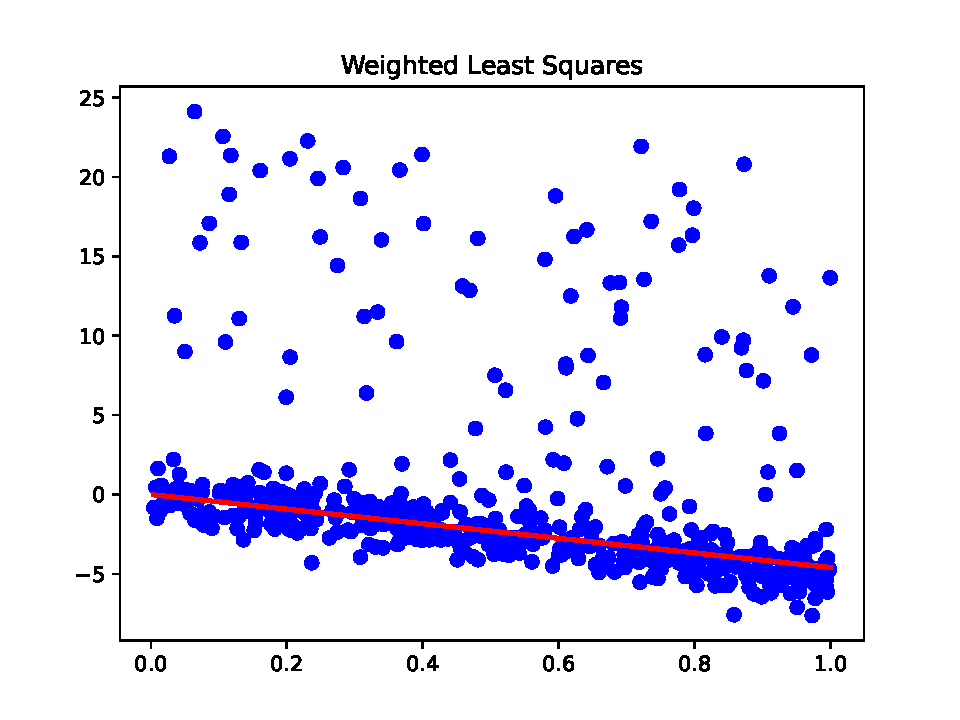
\includegraphics[width = .7\textwidth]{figs/Weighted_least_squares_outliers.pdf}
\end{figure}

\subsection{Smooth Approximation to the L1-Norm \pts{8}}

Unfortunately, we typically do not know the identities of the outliers. In situations where we suspect that there are outliers, but we do not know which examples are outliers, it makes sense to use a loss function that is more robust to outliers. In class, we discussed using the sum of absolute values objective,
\[
f(w) = \sum_{i=1}^n |w^Tx_i - y_i|.
\]
This is less sensitive to outliers than least squares, but it is non-differentiable and harder to optimize. Nevertheless, there are various smooth approximations to the absolute value function that are easy to optimize. One possible approximation is to use the log-sum-exp approximation of the max function\footnote{Other possibilities are the Huber loss, or $|r|\approx \sqrt{r^2+\epsilon}$ for some small $\epsilon$.}:
\[
|r| = \max\{r, -r\} \approx \log(\exp(r) + \exp(-r)).
\]
Using this approximation, we obtain an objective of the form
\[
f(w) {=} \sum_{i=1}^n  \log\left(\exp(w^Tx_i - y_i) + \exp(y_i - w^Tx_i)\right).
\]
which is smooth but less sensitive to outliers than the squared error. \ask{Derive
 the gradient $\nabla f$ of this function with respect to $w$. You should show your work but you do \underline{not} have to express the final result in matrix notation.}

\begin{answer}
	\begin{equation}
		\begin{split}
			\nabla f(w) &= \sum_i^n \frac{x_i(exp(w^{T}x_i - y_i)- exp(y_i - w^{T}x_i)}{\exp(w^Tx_i - y_i) + \exp(y_i - w^Tx_i)} \\
			&= \sum_i^n \frac{x_i(exp(2w^{T}x_i)- exp(2y_i))}{exp(2w^{T}x_i) + exp(2y_i)}
		\end{split}
	\end{equation}
\end{answer}

\subsection{Gradient Descent: Understanding the Code \pts{5}}

Recall gradient descent, a derivative-based optimization algorithm that uses gradients to navigate the parameter space until a locally optimal parameter is found. In \texttt{optimizers.py}, you will see our implementation of gradient descent, taking the form of a class named \texttt{OptimizerGradientDescent}. This class has a similar design pattern as PyTorch, a popular differentiable programming and optimization library. One step of gradient descent is defined as
\[
	w^{t+1} = w^t - \alpha^t \nabla_w f(w^t)
.\]

Look at the methods named \texttt{get\_learning\_rate\_and\_step()} and \texttt{break\_yes()}, and \ask{answer each of these questions, one sentence per answer:}
\begin{enumerate}
	\item Which variable is equivalent to $\alpha^t$, the step size at iteration $t$?
	\begin{answer}
		The variable \texttt{alpha} or \texttt{learning\_rate} is equivalent to the step size
	\end{answer}
	\item Which variable is equivalent to $\nabla_w f(w^t)$ the current value of the gradient vector?
	\begin{answer}
		\texttt{g\_new} is the current gradient vector
	\end{answer}
	\item Which variable is equivalent to $w^t$, the current value of the parameters?
	\begin{answer}
		\texttt{w\_new} is the current parameter
	\end{answer}
	\item What is the method \texttt{break\_yes()} doing?
	\begin{answer}
		It tells whether the iteration should stop based on the current gradient and the maximum number of iterations
	\end{answer}
\end{enumerate}


\subsection{Robust Regression \pts{20}}

The class \texttt{LinearModelGradientDescent} is the same as \texttt{LeastSquares}, except that it fits the least squares model using a gradient descent method. If you run \verb|python main.py -q 2.4| you'll see it produces the same fit as we obtained using the normal equations.

% One advantage of the gradient descent strategy is that it only costs $O(nd)$ for an iteration of the gradient method, which is faster than forming $X^TX$ which costs $O(nd^2)$. Of course, we need to know the \emph{number} of gradient iterations in order to precisely compare these two strategies, but for now we will assume that the number of gradient iterations is typically often reasonable.

The typical input to a gradient method is a function that, given $w$, returns $f(w)$ and $\nabla f(w)$. See \texttt{funObj} in \texttt{LinearModelGradientDescent} for an example. Note that the \texttt{fit} function of \texttt{LinearModelGradientDescent} also has a numerical check that the gradient code is approximately correct, since implementing gradients is often error-prone.\footnote{Sometimes the numerical gradient checker itself can be wrong. See CPSC 303 for a lot more on numerical differentiation.}

An advantage of gradient-based strategies is that they are able to solve
problems that do not have closed-form solutions, such as the formulation from the
previous section. The class \texttt{LinearModelGradientDescent} has most of the implementation
of a gradient-based strategy for fitting the robust regression model under the log-sum-exp approximation.

\subsubsection{Implementing the Objective Function \pts{15}}

Optimizing robust regression parameters is the matter of implementing a function object and using an optimizer to minimize the function object. The only part missing is the function and gradient calculation inside \texttt{fun\_obj.py}.
\ask{Inside \texttt{fun\_obj.py}, complete \texttt{FunObjRobustRegression} to implement the objective function and gradient based on the smooth
approximation to the absolute value function (from the previous section). Hand in your code, as well
as the plot obtained using this robust regression approach.}
\begin{minted}{python}
	class FunObjRobustRegression(FunObj):
		def evaluate(self, w, X, y):
			#Need to use log and exp funtion 
			import math

			# help avoid mistakes (as described in the assignment) by
			# potentially reshaping our arguments
			w = ensure_1d(w)
			y = ensure_1d(y)


			#Define results
			n,d = X.shape
			f = 0
			g = 0

			#Use loop to compute the sumation results
			for i in range(n):
				yi = y[i]
				xi = X[i]
				yi_hat = xi @ w
				residual = yi_hat - yi
				f += math.log(math.exp(residual) + math.exp(-residual))
				g += xi * (math.exp(2*yi_hat) - math.exp(2*yi))/(math.exp(2*yi_hat) + math.exp(2*yi))

			return f,g 
	\end{minted}


	\begin{figure}
		\centering
		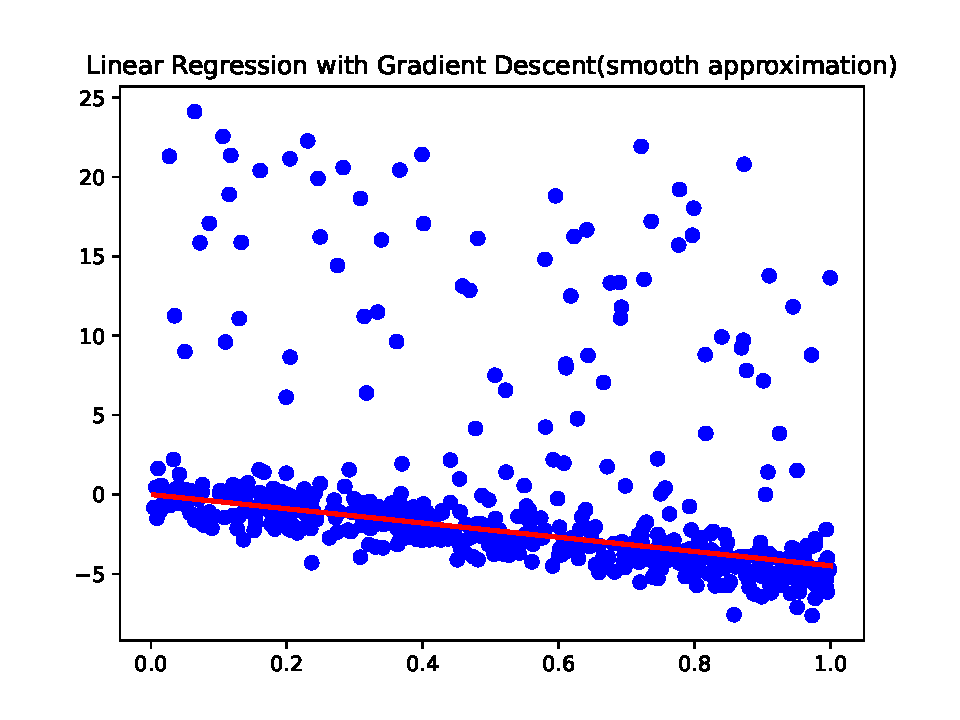
\includegraphics[width = .7\textwidth]{figs/least_squares_robust.pdf}
	\end{figure}

\subsubsection{The Learning Curves \pts{5}}

Using the same dataset as the previous sections, produce the plot of ``gradient descent learning curves'' to compare the performances of \texttt{OptimizerGradientDescent} and \texttt{OptimizerGradientDescentLineSearch} for robust regression, where \textbf{one hundred (100) iterations} of gradient descent are on the x-axis and the \textbf{objective function value} corresponding to each iteration is visualized on the y-axis (see gradient descent lecture). Use the default \texttt{learning\_rate} for \texttt{OptimizerGradientDescent}. \ask{Submit this plot. According to this plot, which optimizer is more ``iteration-efficient''?}

\begin{figure}
	\centering
	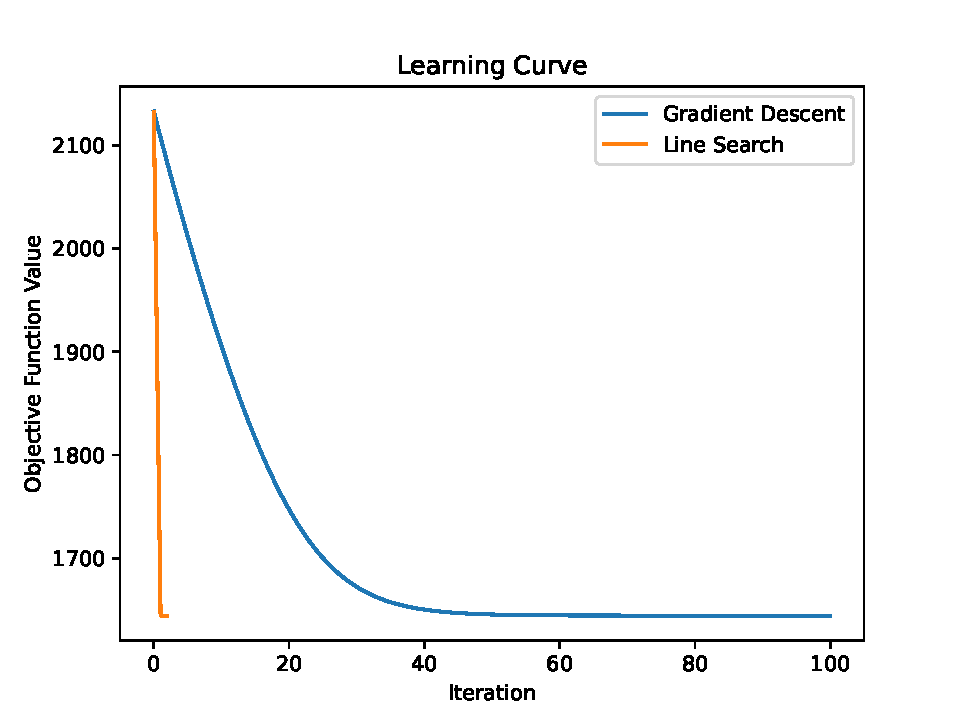
\includegraphics[width = 0.7\textwidth]{figs/LearningCurve.pdf}
\end{figure}

\begin{answer}
	From the graph, the normal gradient descent optimizer arrives around the minimum value after 40 iterations. However, since the iteration didn't stop, the objective funciton can still be minimized. However, the line search optimizer arrives at the minimum value and stopped accroding to our tolerance with 4 iterations. It's clear that the line search optimizer is more efficient in terms of iterations.
\end{answer}
\clearpage
\section{Linear Regression and Nonlinear Bases}

In class we discussed fitting a linear regression model by minimizing the squared error.
% This classic model is the simplest version of many of the more complicated models we will discuss in the course.
% However, it typically performs very poorly in practice.
% One of the reasons it performs poorly is that it assumes that the target $y_i$ is a linear function of
% the features $x_i$ with an intercept of zero. This drawback can be addressed
% by adding a bias (a.k.a. intercept) variable
%  and using nonlinear bases (although nonlinear bases may increase to over-fitting).
In this question, you will start with a data set where least squares performs poorly.
You will then explore how adding a bias variable and using nonlinear (polynomial) bases can drastically improve the performance.
You will also explore how the complexity of a basis affects both the training error and the validation error.
% In the final part of the question, it will be up to you to design a basis with better performance than polynomial bases.

\subsection{Adding a Bias Variable \pts{8}}

\label{biasvar}
If you run  \verb|python main.py -q 3|, it will:
\begin{enumerate}
\item Load a one-dimensional regression dataset.
\item Fit a least-squares linear regression model.
\item Report the training error.
\item Report the validation error.
\item Draw a figure showing the training data and what the linear model looks like.
\end{enumerate}
Unfortunately, this is an awful model of the data. The average squared training error on the data set is over 28000
(as is the validation error), and the figure produced by the demo confirms that the predictions are usually nowhere near
 the training data:
\centerfig{.5}{./figs/least_squares_no_bias.pdf}
The $y$-intercept of this data is clearly not zero (it looks like it's closer to $200$),
so we should expect to improve performance by adding a \emph{bias} (a.k.a. intercept) variable, so that our model is
\[
y_i = w^Tx_i + w_0.
\]
instead of
\[
y_i = w^Tx_i.
\]
\ask{In file \texttt{linear\string_models.py}, complete the class \texttt{LeastSquaresBias},
that has the same input/model/predict format as the \texttt{LeastSquares} class,
but that adds a \emph{bias} variable (also called an intercept) $w_0$ (also called $\beta$ in lecture). Hand in your new class, the updated plot,
and the updated training/validation error.}

Hint: recall that adding a bias $w_0$ is equivalent to adding a column of ones to the matrix $X$. Don't forget that you need to do the same transformation in the \texttt{predict} function.

\begin{minted}{python}
class LeastSquaresBias:
    def fit(self, X, y):
        n,d = X.shape
        one = np.ones((n,1))
        X_reg = np.append(one, X, axis=1)
        LeastSquares.fit(self, X_reg, y)

    def predict(self, X_pred):
        n,d = X_pred.shape
        one = np.ones((n,1))
        X_reg = np.append(one, X_pred, axis=1)
        y_pred= LeastSquares.predict(self,X_reg)

        return y_pred
\end{minted}

\begin{figure}
	\centering
	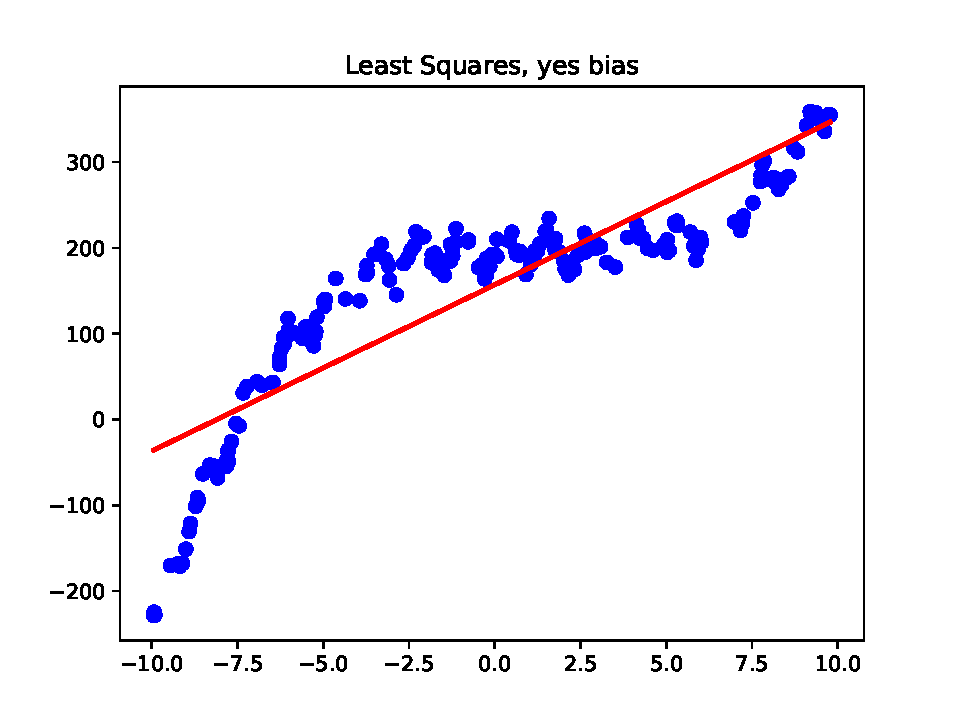
\includegraphics[width = .7\textwidth]{figs/least_squares_yes_bias.pdf}
\end{figure}

\subsection{Polynomial Basis \pts{10}}

Adding a bias variable improves the prediction substantially, but the model is still problematic because the target seems to be a \emph{non-linear} function of the input.
Complete \texttt{LeastSquarePoly} class, that takes a data vector $x$ (i.e., assuming we only have one feature) and the polynomial order $p$. The function should perform a least squares fit based on a matrix $Z$ where each of its rows contains the values $(x_{i})^j$ for $j=0$ up to $p$. E.g., \texttt{LeastSquaresPoly.fit(x,y)}  with $p = 3$ should form the matrix
\[
Z =
\left[\begin{array}{cccc}
1 & x_1 & (x_1)^2 & (x_1)^3\\
1 & x_2 & (x_2)^2 & (x_2)^3\\
\vdots\\
1 & x_n & (x_n)^2 & (x_N)^3\\
\end{array}
\right],
\]
and fit a least squares model based on it.
\ask{Submit your code, and a plot showing training and validation error curves for the following values of $p$: $0,1,2,3,4,5,10,20,30,50,75,100$. Clearly label your axes, and use a logarithmic scale for $y$} by \texttt{plt.yscale("log")} or similar, so that we can still see what's going on if there are a few extremely large errors. \ask{Explain the effect of $p$ on the training error and on the validation error.}

NOTE: large values of $p$ may cause numerical instability. Your solution may look different from others' even with the same code depending on the OS and other factors. As long as your training and validation error curves behave as expected, you will not be penalized.

Note: you should write the code yourself; don't use a library like sklearn's \texttt{PolynomialFeatures}.

Note: in addition to the error curves, the code also produces a plot of the fits themselves. This is for your information; you don't have to submit it.
\begin{answer}
	It can be seen from the figure that, with the increasing of the degree of polinomial, the traning error and validation error are decreasing at the same time at the beginning. However, after 10th degree, the validation error starts to increase dramatically, while the training error is still slowly decreasing. 

	The reason behind the increase of validation error is overfitting into the training data. As $p$ increase, the fitted value is getting more and more closer to the real value during the training. Therefore, it more precisely captures the trend of the training data. This leads to overfitting issue when we use the testing data, and thus cause the validation error to increase.
\end{answer}

\begin{minted}{python}
	class LeastSquaresPoly:
		def __init__(self, p):
			self.leastSquares = LeastSquares()
			self.p = p

		def fit(self, X, y):
			X_reg = LeastSquaresPoly._poly_basis(self, X)
			LeastSquares.fit(self, X_reg, y)


		def predict(self, X_pred):
			X_reg = LeastSquaresPoly._poly_basis(self, X_pred)

			y_pred= LeastSquares.predict(self,X_reg)

			return y_pred

		#Define the polynomial basis
		def _poly_basis(self, X):
			n,d = X.shape
			Z_old = np.ones((n,1))
			Z_new = Z_old
			for i in range(self.p):
				Z_new = np.append(Z_old, np.power(X,i+1),axis = 1)
				Z_old = Z_new
			self.Z = Z_new
			return self.Z
\end{minted}

\begin{figure}
	\centering
	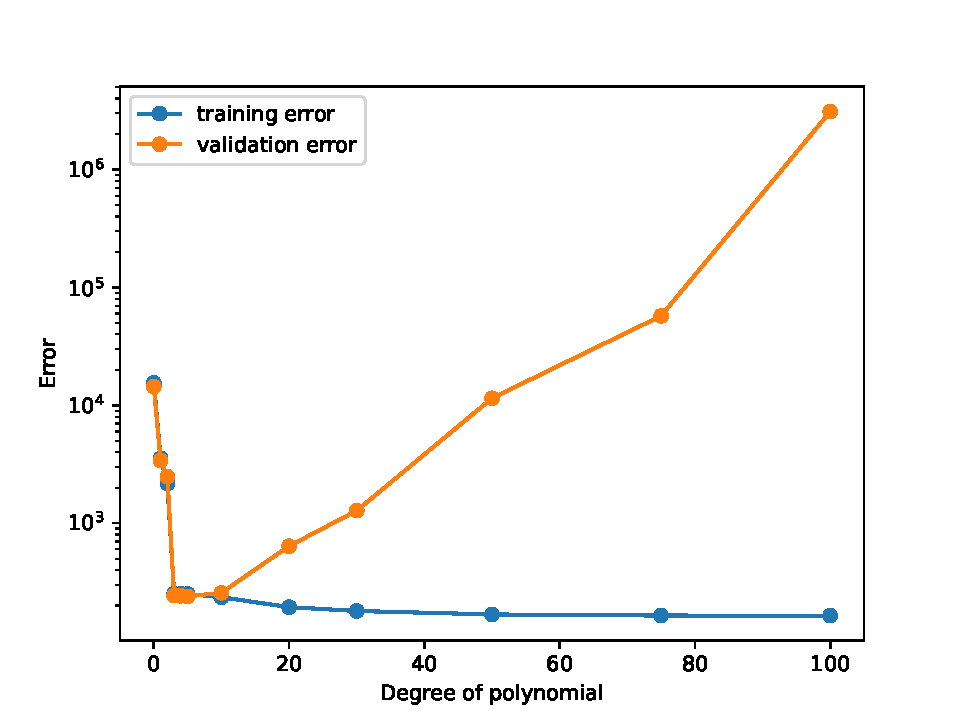
\includegraphics[width = .7\textwidth]{figs/polynomial_error_curves.pdf}
\end{figure}

\clearpage
\section{Very-Short Answer Questions \pts{24}}

\ask{Answer the following questions (in a sentence or two).}

\begin{enumerate}
\item Suppose that a training example is global outlier, meaning it is really far from all other data points. How is the cluster assignment of this example set by $k$-means? And how is it set by density-based clustering?
\begin{answer}
	K-mean method would classify it as the nearest cluster, while the density-based clustering would set itself as a new group.
\end{answer}
%
\item Why do we need random restarts for $k$-means but not for density-based clustering?
\begin{answer}
	Because the $k$-mean can potentially gives different results according to different starting points, while the density-based clustering would always give the same result.

\end{answer}
\item Can hierarchical clustering find non-convex clusters?
\begin{answer}
	It can, since it's essentially density-based clustering
\end{answer}
\item For model-based outlier detection, list an example method and problem with identifying outliers using this method.
\begin{answer}
	We can assume that the data follows a normal distribution and select outlier based on the probability. However, it can be problematic if the data is not normally distributed. For example, the data can be uniformally distributed 
\end{answer}
\item For graphical-based outlier detection, list an example method and problem with identifying outliers using this method.
\begin{answer}
	We could plot the data as a scatter plot, and detect outliers by personal observation. But sometimes it can be hard to tell which points are outliers just based on observation, especially when the data itself is distributed sparsely. 
\end{answer}
\item For supervised outlier detection, list an example method and problem with identifying outliers using this method.
\begin{answer}
	If we have a dataset including a variable identifying whether this entry is an outlier, then we can use supervised learning to detect other outlier in other dataset. However, normally we don't have that kind of data. Moreover, the pattern of outliers can be different, so we can end up with a high testing error.
\end{answer}
\item If we want to do linear regression with 1 feature, explain why it would or would not make sense to use gradient descent to compute the least squares solution.
\begin{answer}
	Still we can use gradient descent, but a closed-form solution can be more computational efficient/
\end{answer}
\item Why do we typically add a column of $1$ values to $X$ when we do linear regression? Should we do this if we're using decision trees?
\begin{answer}
	Because normally we could expect the intercept of fitted value to be non-zero.
\end{answer}
\item Why do we need gradient descent for the robust regression problem, as opposed to just using the normal equations? Hint: it is NOT because of the non-differentiability. Recall that we used gradient descent even after smoothing away the non-differentiable part of the loss.
\begin{answer}
	Firstly, normal equation can only solve linear problems. Secondly, gradient descent potentially is computational efficient.
\end{answer}
%
\item What is the problem with having too small of a learning rate in gradient descent? What is the problem with having too large of a learning rate in gradient descent?
\begin{answer}
	It would cost more iterations to find the optimal with too small a learning rate. While it may not coverge if the learning rate is too large.
\end{answer}
\item What is the purpose of the log-sum-exp function and how is this related to gradient descent?
\begin{answer}
	It smoothes the objective function so that we can find the gradient.
\end{answer}
\item What type of non-linear transform might be suitable if we had a periodic function?
\begin{answer}
	We can use trigonometric functions like sines and cosines.
\end{answer}
\end{enumerate}

\end{document}
